\documentclass[spanish, c]{beamer}

\usepackage[utf8]{inputenc}
% \usepackage[spanish, mexico]{babel}
\usepackage{amsmath}
\usepackage{mathtools}
\usepackage{hyperref}
\usepackage{xcolor}
\usepackage{color}
\usepackage{ragged2e}
\usepackage{mathrsfs}
% \usepackage{csquotes}
% \usepackage{listings}
\usepackage[scaled]{beramono}
\usepackage[T1]{fontenc}
\usepackage{graphicx}
\usepackage{booktabs}
% \usepackage{physics}
% \usepackage{minted}
\usepackage{tcolorbox}
\usepackage{tikz}
\usepackage{relsize}
\usepackage{algorithm}
\usepackage{algpseudocode}
\usepackage{pifont}

\newcommand{\cmark}{\ding{51}}%
\newcommand{\xmark}{\ding{55}}%

\tcbuselibrary{minted, skins}

\usetikzlibrary{arrows, automata, positioning, fit, shapes.geometric, backgrounds}
  
  \tikzset{
    stylename/.style={
      ->, %arrow type
      >=stealth', %arrow head type (bold)
      shorten >=1pt, 
      auto,
      %semithick,
      initial text=$ $, %no start text
    }
  }

\renewcommand{\indent}{\hspace*{2em}}

\newcommand\CC{C\nolinebreak[4]\hspace{-.05em}\raisebox{.4ex}{\relsize{-3}{\textbf{++}}}~}
\newcommand{\bigO}{\mathcal{O}}

\renewcommand{\Comment}[2][.55\linewidth]{%
  \leavevmode\hfill\makebox[#1][l]{\fontfamily{cmss}\selectfont\color{red}\footnotesize$\longrightarrow$\quad#2}}
% \usepackage{tikz}

% \usetikzlibrary{fit, shapes, arrows}

% \usepackage{courier}
% \usepackage{subfigure}
% \usepackage{enumerate}
% \usepackage{algorithmic}
% \usepackage{algorithm}

% \usepackage{listings}
% \usepackage{lstlinebgrd}

\usetheme{Boadilla}
\usefonttheme[onlymath]{serif}

\newcommand\blfootnote[1]{%
\begingroup
\renewcommand\thefootnote{}\footnote{#1}%
\addtocounter{footnote}{-1}%
\endgroup
}

\algrenewcommand\alglinenumber[1]{\footnotesize #1}

\makeatletter
% start with some helper code
% This is the vertical rule that is inserted
\newcommand*{\algrule}[1][\algorithmicindent]{%
  \makebox[#1][l]{%
    \hspace*{.2em}% <------------- This is where the rule starts from
    \vrule height .75\baselineskip depth .25\baselineskip
  }
}

\newcount\ALG@printindent@tempcnta
\def\ALG@printindent{%
    \ifnum \theALG@nested>0% is there anything to print
    \ifx\ALG@text\ALG@x@notext% is this an end group without any text?
    % do nothing
    \else
    \unskip
    % draw a rule for each indent level
    \ALG@printindent@tempcnta=1
    \loop
    \algrule[\csname ALG@ind@\the\ALG@printindent@tempcnta\endcsname]%
    \advance \ALG@printindent@tempcnta 1
    \ifnum \ALG@printindent@tempcnta<\numexpr\theALG@nested+1\relax
    \repeat
    \fi
    \fi
}
% the following line injects our new indent handling code in place of the default spacing
\patchcmd{\ALG@doentity}{\noindent\hskip\ALG@tlm}{\ALG@printindent}{}{\errmessage{failed to patch}}
\patchcmd{\ALG@doentity}{\item[]\nointerlineskip}{}{}{} % no spurious vertical space
% end vertical rule patch for algorithmicx
\makeatother
%

% Sets the templates
\definecolor{navyblue}{RGB}{0, 0, 128}
\definecolor{crimson}{RGB}{128, 16, 0}

\setbeamertemplate{navigation symbols}{}
\setbeamertemplate{headline}{}
\setbeamertemplate{title page}[default][colsep=-4bp,rounded=true]
\setbeamertemplate{footline}[frame number]
\setbeamertemplate{bibliography item}[text]
\setbeamertemplate{theorems}[numbered]

\setbeamercolor{title}{fg=navyblue, bg=white}
\setbeamercolor{frametitle}{fg=navyblue, bg=white}
\setbeamercolor{structure}{fg=navyblue}
\setbeamercolor{button}{fg=white,bg=navyblue}

\setbeamercovered{transparent}

\tcbset{cppexample/.style={%
    colback=green!5,
    colframe=green!30!black,
    listing only,
    fonttitle=\bfseries,
    listing engine=minted,
    minted language=c++,
    minted options={fontsize=\scriptsize, breaklines, linenos, autogobble, numbersep=2mm},
    enhanced,
    overlay={\begin{tcbclipinterior}\fill[red!25!green!25!white] (frame.south west)rectangle ([xshift=4mm]frame.north west);\end{tcbclipinterior}}
}}

\tcbset{cppfullexample/.style={%
    % colback=green!5,
    % colframe=green!30!black,
    listing only,
    fonttitle=\bfseries,
    listing engine=minted,
    minted language=c++,
    minted options={fontsize=\scriptsize, breaklines, linenos, autogobble, numbersep=2mm},
    enhanced,
    overlay={\begin{tcbclipinterior}\fill[black!20!white] (frame.south west)rectangle ([xshift=4mm]frame.north west);\end{tcbclipinterior}}
}}

\tcbset{cppfullborderless/.style={%
    % colback=green!5,
    % colframe=green!30!black,
    listing only,
    listing engine=minted,
    minted language=c++,
    minted options={fontsize=\scriptsize, breaklines, linenos, autogobble, numbersep=2mm},
    enhanced,
    overlay={\begin{tcbclipinterior}\fill[black!20!white] (frame.south west)rectangle ([xshift=4mm]frame.north west);\end{tcbclipinterior}}
}}

\title{Conceptos matemáticos preliminares}
\subtitle{Implementación de Métodos Computacionales \\ (TC2037)}
\author{
    \texorpdfstring{
        \begin{center}
            M.C. Xavier Sánchez Díaz \\
            \href{mailto:mail@tec.mx}{\texttt{mail@tec.mx}}
        \end{center}
    }
    {M.C. Xavier Sánchez Díaz}
}

\institute[Tecnológico de Monterrey]{
\includegraphics[scale=0.5]{../img/logo}}
\date{}

\begin{document}

\setlength{\rightskip}{0pt}

\begin{frame}[plain]
    \titlepage        
\end{frame}

\begin{frame}{Outline}
    \tableofcontents
\end{frame}

\section{Conjuntos}
\label{sec:conjuntos}

\begin{frame}{Definición de conjunto}{Conjuntos}
    \begin{definition}
        Un \alert{conjunto} es una colección de elementos.
        Usamos letras mayúsculas $A, B, C, \dots$ para representarlos, y letras minúsculas $a, b, c, \dots$ para representar sus elementos.
    \end{definition}
    \bigskip
    \[A = \{a, b, c, d\}\]
\end{frame}

\begin{frame}{Describiendo un conjunto}{Conjuntos}
    Podemos definirlos por \textit{enumeración} o por \textit{descripción}. \pause
    \bigskip
    \begin{center}
        $A$ es el conjunto de todos los números naturales menores que 6. \pause
    \end{center}

    \begin{exampleblock}{Enumerando sus elementos}
        $A = \{1, 2, 3, 4, 5\} = \{2, 3, 1, 5, 4\}$
    \end{exampleblock} \pause

    \begin{exampleblock}{Describiendo sus elementos}
        $A = \{a \in \mathbb{N} : a < 6\}$
    \end{exampleblock}
\end{frame}

\begin{frame}{Notación de conjuntos}{Conjuntos}
    \begin{itemize}
    \justifying
    \itemsep1.5em
        \item <1-> \textbf{Pertenencia}: $a \in A$, cuando $a$ es un elemento de $A$.
        \item <2-> \textbf{Cardinalidad}: $|A|$ representa el número de elementos en $A$.
        \item <3-> \textbf{Inclusión}: $A \subseteq B$ si todos los elementos de $A$ son elementos de $B$.
        \item <4-> \textbf{Igualdad}: si $A \subseteq B$ y $B \subseteq A$, entonces $A = B$.
        \item <5-> \textbf{Inclusión propia}: $A \subset B$ si todos los elementos de $A$ son elementos de $B$ y $A \neq B$.
        \item <6-> \textbf{Conjunto vacío}: $\varnothing$ o $\{\}$ para representar un conjunto sin elementos.
    \end{itemize}
\end{frame}

\begin{frame}{Pertenencia e inclusión}{Conjuntos}
    \begin{columns}
        \begin{column}{0.5\textwidth}
        \begin{enumerate}
            \itemsep1.5em
            \item <1,11> \alert<11>{$\{a\} \subseteq \{\{a\}\}$}
            \item <2,11> \alert<11>{$\{a\} \subseteq \{b, c, \{a\}\}$}
            \item <3,11> \alert<11>{$a \subseteq \{a, b, c\}$}
            \item <4,11> $\{a\} \in \{b,c, \{a\}\}$
            \item <5,11> $a \in \{a,b,c\}$
        \end{enumerate}
        \end{column}

        \begin{column}{0.5\textwidth} 
        \begin{enumerate}
            \itemsep1.5em
            \setcounter{enumi}{5}
            \item <6,11> $\{b\} \in \{a, c, \{b\}\}$
            \item <7,11> $b \in \{b\}$
            \item <8,11> \alert<11>{$\{b\} \subseteq \{\{b,c\}\}$}
            \item <9,11> \alert<11>{$\{b\} \subseteq \{\{a\}, c, \{b\}\}$}
            \item <10,11> $\{c\} \subset \{\{a\}, c, \{b\}\}$
        \end{enumerate}
        \end{column}
    \end{columns}
\end{frame}

\begin{frame}{Conjunto vacío}{Conjuntos}
    \begin{enumerate}
        \itemsep1.5em
        \item <1,6> $\varnothing \subset \{\varnothing\}$ 
        \item <2,6> $\varnothing \in \{\varnothing\}$
        \item <3,6> \alert<6>{$0 = \varnothing$}
        \item <4,6> $\varnothing \subseteq \varnothing$
        \item <5,6> \alert<6>{$\varnothing \subset \varnothing$}
    \end{enumerate}
\end{frame}

\begin{frame}{Operaciones de conjuntos}{Conjuntos} 
    \def \setA{(-0.7, 0) circle (1)}
    \def \setB{(0.7, 0) circle (1)}
    \def \setC{(0, -1) circle (1)}

    \begin{columns}
        \begin{column}{0.5\textwidth}
            \begin{tikzpicture}
                \draw (-2, 1.5) rectangle (2, -2.5);
                \draw[color=red, line width=1pt] \setA node[above left] {$A$};
                \draw[color=blue, line width=1pt] \setB node[above] {$B$};
                \draw[color=green, line width=1pt] \setC node[below] {$C$};
            \end{tikzpicture}
        \end{column}
        \begin{column}{0.5\textwidth}
            \begin{enumerate}
                \item <1> $B \cup C$
                \item <2> $C \cup (A \cap B)$
                \item <3> $C - (A \cap B)$
                \item <4> $A - (B \cup C)$
                \item <5> $A^\complement$
                \item <6> $B - (A \cup C)$
                \item <7> $(B - A)^\complement$
            \end{enumerate}
        \end{column}
    \end{columns}
\end{frame}

\begin{frame}{Producto Cartesiano}{Conjuntos}
    \begin{definition}
        El \alert{producto Cartesiano} entre $A$ y $B$ se define como:
        \[A \times B = \{(x,y) : x \in A, y \in B\}\] 
    \end{definition}
        \pause
    \begin{exampleblock}{Ejemplo}
        \vspace{-2.5ex}
        \begin{align*}
        \onslide<2->{& A = \{1,2,3\} \quad B = \{1,2\}\\}
        \onslide<3->{A \times B & = \{(1,1), (1,2), (2,1), (2,2), (3,1), (3,2)\}}
        \end{align*}
    \end{exampleblock}
        \onslide<4->{\[|A \times B| = |A| \times |B|\]}
\end{frame}

\begin{frame}{Conjunto potencia}{Conjuntos}
    \begin{definition}
        Sea $A$ cualquier conjunto. El \alert{conjunto potencia} de $A$---denotado por $\mathscr{P}(A)$ o $\wp(A)$---consiste en el conjunto de todos (y únicamente) los subconjuntos de $A$.
    \end{definition}
    \pause
    \bigskip
    \[\mathscr{P}(\{a,b,c\}) = \{\varnothing, \{a\}, \{b\}, \{c\}, \{a,b\}, \{a,c\}, \{b,c\}, \{a,b,c\}\}\] \pause
    \bigskip
    \[|\mathscr{P}(A)| = 2^{|A|}\]
\end{frame}

\begin{frame}{Equivalencias}{Conjuntos}
    \label{fr:equivalence}
    La \textbf{unión} y la \textbf{intersección} son \alert{conmutativas}. \pause
    \bigskip
    \[A \cup B = B \cup A\] \pause
    \bigskip
    \[A \cap B = B \cap A\]
\end{frame}

\begin{frame}{Equivalencias}{Conjuntos}
    La \textbf{unión} y la \textbf{intersección} son \alert{asociativas}. \pause
    \bigskip
    \[(A \cup B) \cup C = A \cup (B \cup C)\] \pause
    \bigskip
    \[(A \cap B) \cap C = A \cap (B \cap C)\]
\end{frame}

\begin{frame}{Equivalencias}{Conjuntos}
    La \textbf{unión} y la \textbf{intersección} son \alert{distributivas} entre ellas. \pause
    \bigskip
    \[A \cup (B \cap C) = (A \cup B) \cap (A \cup C)\] \pause
    \bigskip
    \[A \cap (B \cup C) = (A \cap B) \cup (A \cap C)\]
\end{frame}

\begin{frame}{Equivalencias}{Conjuntos}
    Leyes de \alert{De Morgan}: \pause
    \bigskip
    \[(A \cup B)^\complement = A^\complement \cap B^\complement\] \pause
    \[(A \cap B)^\complement = A^\complement \cup B^\complement\]
    \bigskip
    \hyperlink{fr:logicequiv}{\beamergotobutton{Slide de Lógica}}
\end{frame}

\section{Relaciones y Funciones}
\label{sec:relfunc}

\begin{frame}{Relaciones}{Relaciones y Funciones}
    \begin{definition}
        Sean $A$ y $B$ dos conjuntos cualesquiera. Una \alert{relación binaria} $R$ \textit{de} $A$ \textit{a} $B$ se define como cualquier subconjunto del producto Cartesiano $A \times B$.
        Es decir, cualquier conjunto de pares ordenados de la forma $(a,b)$ tal que $a \in A$ y $b \in B$.
        También se dice que una relación $R$ puede ser \textit{sobre} $A \times B$.
    \end{definition} \pause
    \bigskip
    \begin{exampleblock}{Ejemplo}
        \textit{Menor o igual} ($\leq$) es una \textbf{relación} sobre $\mathbb{N} \times \mathbb{N}$:
        \[\leq \, = \{(1,1), (1,2), (1,3), \dots , (2,2), (2,3), \dots , (3,4), \dots \}\]
    \end{exampleblock}
\end{frame}

\begin{frame}{Reflexividad}{Relaciones y funciones}

    \begin{definition}
        Sea $R$ una relación binaria. Se dice que es \alert{reflexiva} sobre un conjunto $A$ si y solo si $(a,a) \in R$ para todo $a \in A$.
    \end{definition} \pause
    \bigskip
    \begin{exampleblock}{Ejemplo}
        \textit{Menor o igual} ($\leq$) es una relación \textbf{reflexiva} sobre $\mathbb{N} \times \mathbb{N}$:
        \[\leq \, = \{\mathbf{(1,1)}, (1,2), (1,3), \dots , \mathbf{(2,2)}, (2,3), \dots , (3,4), \dots \}\]
    \end{exampleblock} \pause
    \bigskip
    ¿Es la relación \textit{menor que} $(<)$ reflexiva sobre los naturales?
\end{frame}

\begin{frame}{Reflexividad}{Relaciones y funciones}
    \begin{center}
        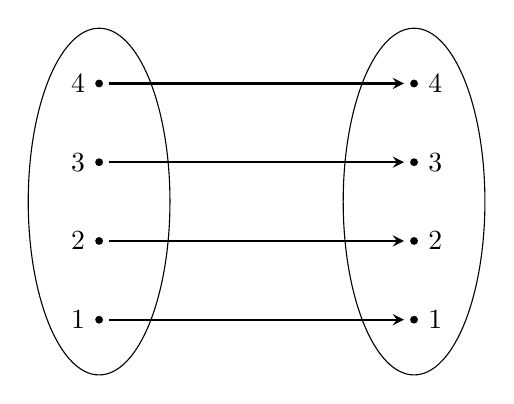
\begin{tikzpicture}[
            >=stealth,
            bullet/.style={
              fill=black,
              circle,
              minimum width=1pt,
              inner sep=1pt
            },
            projection/.style={
              ->,
              thick,
              shorten <=2pt,
              shorten >=2pt
            },
            every fit/.style={
              ellipse,
              draw,
              inner sep=0pt
            }
          ]
            \foreach \y/\l in {1/d,2/c/,3/b,4/a}
              \node[bullet,label=left:$\y$] (a\y) at (0,\y) {};
        
            \foreach \y/\l in {1/1,2/2,3/3,4/4}
              \node[bullet,label=right:$\l$] (b\y) at (4,\y) {};
        
            \node[draw,fit=(a1) (a2) (a3) (a4),minimum width=1.8cm] {} ;
            \node[draw,fit=(b1) (b2) (b3) (b4),minimum width=1.8cm] {} ;
        
            \onslide<2->{\draw[projection] (a1) -- (b1);}
            \onslide<3->{\draw[projection] (a2) -- (b2);}
            \onslide<4->{\draw[projection] (a3) -- (b3);}
            \onslide<5->{\draw[projection] (a4) -- (b4);}
          \end{tikzpicture}
    \end{center}
\end{frame}

\begin{frame}{Transitividad}{Relaciones y funciones}
    \begin{definition}
        Decimos que $R$ es \alert{transitiva} si y sólo si cuando $(a,b) \in R$ y $(b,c) \in R$, entonces $(a,c) \in R$.
    \end{definition} \pause
    \bigskip
    \begin{exampleblock}{Ejemplo}
        \textit{Menor o igual} ($\leq$) es una relación \textbf{transitiva} sobre $\mathbb{N} \times \mathbb{N}$:
        \[\leq \, = \{(1,1), \mathbf{(1,2)}, \mathbf{(1,3)}, \dots , (2,2), \mathbf{(2,3)}, \dots , (3,4), \dots \}\]
    \end{exampleblock} \pause
    \bigskip
    ¿Es la relación \textit{menor que} $(<)$ transitiva sobre los naturales?
\end{frame}

\begin{frame}{Transitividad}{Relaciones y funciones}
    \begin{center}
        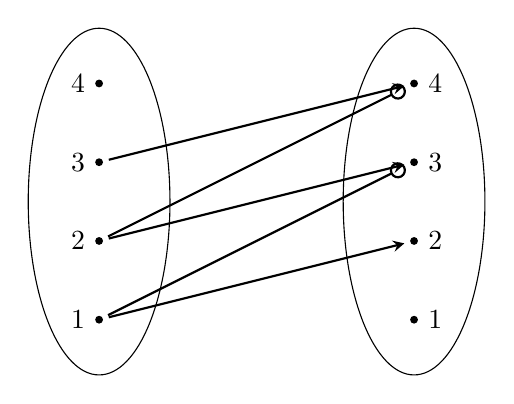
\begin{tikzpicture}[
            >=stealth,
            bullet/.style={
              fill=black,
              circle,
              minimum width=1pt,
              inner sep=1pt
            },
            projection/.style={
              ->,
              thick,
              shorten <=2pt,
              shorten >=2pt
            },
            every fit/.style={
              ellipse,
              draw,
              inner sep=0pt
            },
            projection2/.style={
              -o,
              thick,
              shorten <=2pt,
              shorten >=2pt
            }
          ]
            \foreach \y/\l in {1/d,2/c/,3/b,4/a}
              \node[bullet,label=left:$\y$] (a\y) at (0,\y) {};
        
            \foreach \y/\l in {1/1,2/2,3/3,4/4}
              \node[bullet,label=right:$\l$] (b\y) at (4,\y) {};
        
            \node[draw,fit=(a1) (a2) (a3) (a4),minimum width=1.8cm] {} ;
            \node[draw,fit=(b1) (b2) (b3) (b4),minimum width=1.8cm] {} ;
        
            \onslide<2-4>{\draw[projection] (a1) -- (b2);}
            \onslide<3-4,5->{\draw[projection] (a2) -- (b3);}
            \onslide<4>{\draw[projection2] (a1) -- (b3);}
            \onslide<6->{\draw[projection] (a3) -- (b4);}
            \onslide<7->{\draw[projection2] (a2) -- (b4);}
          \end{tikzpicture}
    \end{center}
\end{frame}

\begin{frame}{Simetría}{Relaciones y funciones}
    \begin{definition}
        Una relación $R$ es \alert{simétrica} si y sólo si cuando $(a,b) \in R$, entonces $(b,a) \in R$.
    \end{definition} \pause
    \bigskip
    \begin{exampleblock}{Ejemplo 1}
        La relación de \textit{igualdad} $(=)$ es una relación \textbf{simétrica}: si $a = b$, entonces $b = a$.
    \end{exampleblock} \pause
    \bigskip
    \begin{exampleblock}{Ejemplo 2}
        La relación de \textit{hermandad} es \textbf{simétrica}: si $Juan$ es hermano de $Pedro$, entonces $Pedro$ es hermano de $Juan$. 
    \end{exampleblock}
\end{frame}

\begin{frame}{Mapeo o Función}{Relaciones y Funciones}
    
    ¿Cualquier relación es una función? \pause
    
    \bigskip

    ¿Cualquier función es una relación?
\end{frame}

\begin{frame}{Mapeo o Función}{Relaciones y Funciones}
    \begin{definition}
        Una \alert{función} \textit{unitaria} de un conjunto $A$ en un conjunto $B$ es cualquier relación binaria $R$ de $A$ a $B$ que satisfaga la condición de que \textit{para todo} $a \in A$ existe \textit{exactamente un} $b \in B$ tal que $(a,b) \in R$.
    \end{definition} \pause
    \bigskip
    Podemos describir una función $f$ de $A$ en $B$ como $f : A \to B$. \pause
    \bigskip
    \begin{exampleblock}{Ejemplo}
        La relación \textit{sucesor} es una \textbf{función} de los naturales en los naturales $f : \mathbb{N} \to \mathbb{N}$
        \[\mathtt{suc}(n) = \{(1,2), (2,3), (3,4), (4,5), \dots\}\]
    \end{exampleblock}
\end{frame}

\begin{frame}{Dominio}{Funciones y Relaciones}
    \begin{definition}
        El \alert{dominio} de una función $f$ puede definirse como
        \[\mathtt{dom}(f) = \{a \in A : \exists b \in B, f(a) = b\}\]
    \end{definition} \pause
    \bigskip
    En una función de forma $f : A \to B$, el \textbf{dominio} es simplemente $A$.
\end{frame}

\begin{frame}{Codominio o Rango}{Funciones y Relaciones}
    \begin{definition}
        El \alert{codominio} (también conocido como \alert{rango}) de una función $f$ puede definirse como
        \[\mathtt{codom}(f) = \{b \in B : \exists a \in A, f(a) = b\}\]
    \end{definition} \pause
    \bigskip
    En una función de forma $f : A \to B$, el \textbf{codominio} es simplemente $B$.    
\end{frame}

\begin{frame}{Funciones totales y parciales}{Relaciones y Funciones}

    \begin{definition}
        Una \alert{función parcial} de un conjunto $A$ a un conjunto $B$ es una relación binaria $R$ de $A$ a $B$ tal que para toda $a \in A$, hay \textit{a lo mucho} un $b \in B$ con $(a,b) \in R$.
    \end{definition} \pause
    \bigskip
    Es decir que puede haber elementos en $A$ que no tengan la relación $R$ a ningún elemento de $B$; o en otras palabras, que no se \textit{usen}. \pause
    
    \bigskip

    A las funciones donde se utilizan \textbf{todos} los elementos de $A$ les llamamos \alert{funciones totales}, y son usualmente a las que nos referimos al simplemente decir ``funciones''.
\end{frame}

\begin{frame}{Funciones Parciales}{Relaciones y funciones}
    \begin{center}
        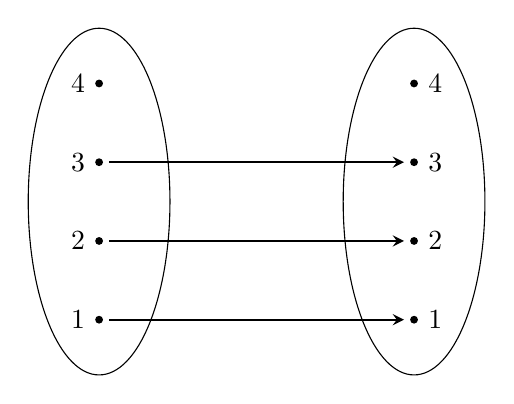
\begin{tikzpicture}[
            >=stealth,
            bullet/.style={
              fill=black,
              circle,
              minimum width=1pt,
              inner sep=1pt
            },
            projection/.style={
              ->,
              thick,
              shorten <=2pt,
              shorten >=2pt
            },
            every fit/.style={
              ellipse,
              draw,
              inner sep=0pt
            }
          ]
            \foreach \y/\l in {1/d,2/c/,3/b,4/a}
              \node[bullet,label=left:$\y$] (a\y) at (0,\y) {};
        
            \foreach \y/\l in {1/1,2/2,3/3,4/4}
              \node[bullet,label=right:$\l$] (b\y) at (4,\y) {};
        
            \node[draw,fit=(a1) (a2) (a3) (a4),minimum width=1.8cm] {} ;
            \node[draw,fit=(b1) (b2) (b3) (b4),minimum width=1.8cm] {} ;
        
            \draw[projection] (a1) -- (b1);
            \draw[projection] (a2) -- (b2);
            \draw[projection] (a3) -- (b3);
          \end{tikzpicture}
    \end{center}
\end{frame}

\begin{frame}{Imagen}{Relaciones y Funciones}
    \begin{definition}
        Sean $f : A \to B$ y $X \subseteq A$. La \alert{imagen} \textit{bajo} $f$ de $X \subseteq A$ es el conjunto $\{b \in B : \exists a \in X, b = f(a)\}$, o bien $\{f(a) : a \in A\}$.
    \end{definition} \pause
    \bigskip
    En otras palabras, la \textbf{imagen} de una función es el conjunto de todos los \textit{valores} de $B$ que \textit{utiliza}.
    \bigskip
    Puede haber elementos de $B$ fuera de la función. Todo $B$ es el \textbf{codominio} de la función, y sólo aquellos $b \in B$ que son usados representan la \textbf{imagen} de la función.
    
\end{frame}

\begin{frame}{Funciones inyectivas}{Relaciones y Funciones}
    \begin{definition}
        Sea $f : A \to B$. Se dice que $f$ es \alert{inyectiva} (o \alert{uno a uno}) si y sólo si cuando $a \neq a'$, entonces $f(a) \neq f(a')$.
    \end{definition} \pause
    \bigskip
    En otras palabras, si y sólo si para cada $b \in B$, hay a lo mucho un $a \in A$ con $f(a) = b$. Es decir, sólo si distintos \textit{inputs} generan \textit{outputs} diferentes.
\end{frame}

\begin{frame}{Funciones inyectivas}{Relaciones y Funciones}
    \begin{center}
        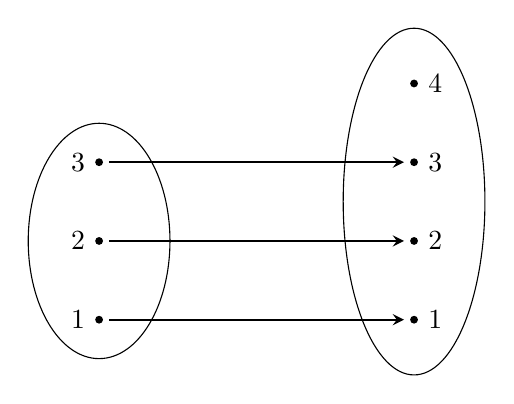
\begin{tikzpicture}[
            >=stealth,
            bullet/.style={
              fill=black,
              circle,
              minimum width=1pt,
              inner sep=1pt
            },
            projection/.style={
              ->,
              thick,
              shorten <=2pt,
              shorten >=2pt
            },
            every fit/.style={
              ellipse,
              draw,
              inner sep=0pt
            }
          ]
            \foreach \y/\l in {1/d,2/c/,3/b}
              \node[bullet,label=left:$\y$] (a\y) at (0,\y) {};
        
            \foreach \y/\l in {1/1,2/2,3/3,4/4}
              \node[bullet,label=right:$\l$] (b\y) at (4,\y) {};
        
            \node[draw,fit=(a1) (a2) (a3),minimum width=1.8cm] {} ;
            \node[draw,fit=(b1) (b2) (b3) (b4),minimum width=1.8cm] {} ;
        
            \draw[projection] (a1) -- (b1);
            \draw[projection] (a2) -- (b2);
            \draw[projection] (a3) -- (b3);
          \end{tikzpicture}
    \end{center}
\end{frame}

\begin{frame}{Funciones inyectivas}{Relaciones y Funciones}
    \begin{center}
        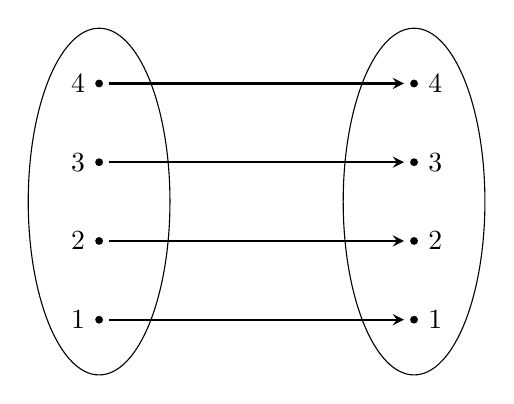
\begin{tikzpicture}[
            >=stealth,
            bullet/.style={
              fill=black,
              circle,
              minimum width=1pt,
              inner sep=1pt
            },
            projection/.style={
              ->,
              thick,
              shorten <=2pt,
              shorten >=2pt
            },
            every fit/.style={
              ellipse,
              draw,
              inner sep=0pt
            }
          ]
            \foreach \y/\l in {1/d,2/c/,3/b,4/d}
              \node[bullet,label=left:$\y$] (a\y) at (0,\y) {};
        
            \foreach \y/\l in {1/1,2/2,3/3,4/4}
              \node[bullet,label=right:$\l$] (b\y) at (4,\y) {};
        
            \node[draw,fit=(a1) (a2) (a3) (a4),minimum width=1.8cm] {} ;
            \node[draw,fit=(b1) (b2) (b3) (b4),minimum width=1.8cm] {} ;
        
            \draw[projection] (a1) -- (b1);
            \draw[projection] (a2) -- (b2);
            \draw[projection] (a3) -- (b3);
            \draw[projection] (a4) -- (b4);
          \end{tikzpicture}
    \end{center}
\end{frame}

\begin{frame}{Funciones sobreyectivas}{Relaciones y Funciones}
    \begin{definition}
        Sea $f : A \to B$. Decimos que $f$ es una función \alert{sobre} $B$ (o \alert{sobreyectiva} con respecto a $B$) si y sólo si para todo $b \in B$ hay algún $a \in A$ con $f(a) = b$.
    \end{definition} \pause
    \bigskip
    Una manera mucho más sencilla de verlo: si y sólo si $\mathtt{imagen}(f) = B$.
\end{frame}

\begin{frame}{Funciones sobreyectivas}{Relaciones y Funciones}
    \begin{center}
        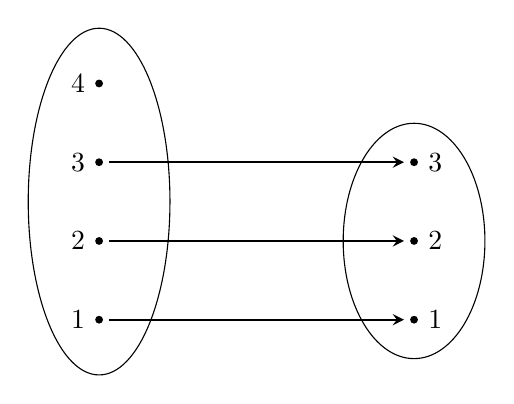
\begin{tikzpicture}[
            >=stealth,
            bullet/.style={
              fill=black,
              circle,
              minimum width=1pt,
              inner sep=1pt
            },
            projection/.style={
              ->,
              thick,
              shorten <=2pt,
              shorten >=2pt
            },
            every fit/.style={
              ellipse,
              draw,
              inner sep=0pt
            }
          ]
            \foreach \y/\l in {1/d,2/c/,3/b,4/d}
              \node[bullet,label=left:$\y$] (a\y) at (0,\y) {};
        
            \foreach \y/\l in {1/1,2/2,3/3}
              \node[bullet,label=right:$\l$] (b\y) at (4,\y) {};
        
            \node[draw,fit=(a1) (a2) (a3) (a4),minimum width=1.8cm] {} ;
            \node[draw,fit=(b1) (b2) (b3), minimum width=1.8cm] {} ;
        
            \draw[projection] (a1) -- (b1);
            \draw[projection] (a2) -- (b2);
            \draw[projection] (a3) -- (b3);
          \end{tikzpicture}
    \end{center}
\end{frame}

\begin{frame}{Funciones biyectivas}{Relaciones y Funciones}
    \begin{definition}
        Se dice que una función es \alert{biyectiva} si y sólo si es \textbf{inyectiva} y \textbf{sobre}.
    \end{definition}
\end{frame}

\begin{frame}{Funciones biyectivas}{Relaciones y Funciones}
    \begin{center}
        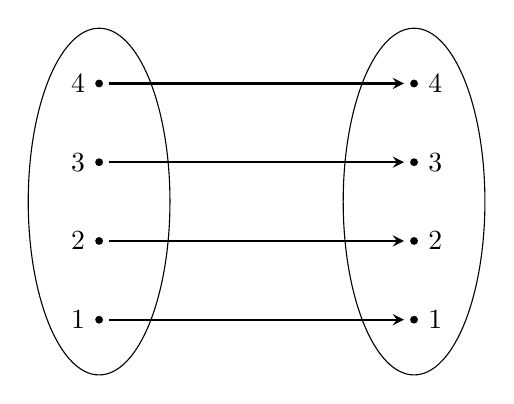
\begin{tikzpicture}[
            >=stealth,
            bullet/.style={
              fill=black,
              circle,
              minimum width=1pt,
              inner sep=1pt
            },
            projection/.style={
              ->,
              thick,
              shorten <=2pt,
              shorten >=2pt
            },
            every fit/.style={
              ellipse,
              draw,
              inner sep=0pt
            }
          ]
            \foreach \y/\l in {1/d,2/c/,3/b,4/d}
              \node[bullet,label=left:$\y$] (a\y) at (0,\y) {};
        
            \foreach \y/\l in {1/1,2/2,3/3,4/4}
              \node[bullet,label=right:$\l$] (b\y) at (4,\y) {};
        
            \node[draw,fit=(a1) (a2) (a3) (a4),minimum width=1.8cm] {} ;
            \node[draw,fit=(b1) (b2) (b3) (b4),minimum width=1.8cm] {} ;
        
            \draw[projection] (a1) -- (b1);
            \draw[projection] (a2) -- (b2);
            \draw[projection] (a3) -- (b3);
            \draw[projection] (a4) -- (b4);
          \end{tikzpicture}
    \end{center}
\end{frame}

\begin{frame}{Conjuntos infinitos}{Relaciones y Funciones}
    \begin{itemize}
        \justifying
        \itemsep1.5em
        \item <1-> Los números \alert{naturales} $\mathbb{N} = \{1, 2, 3, 4, \dots\}$ son infinitos. Algunos autores consideran que $0 \in \mathbb{N}$, otros no. $\mathbb{N}$ es un conjunto infinito \textbf{contable}.
        \item <2-> Los números \alert{enteros} $\mathbb{Z}$ y los números \alert{racionales} $\mathbb{Q}$ son también \textbf{infinitos contables} porque existe una \textbf{biyección} que los empareja uno a uno con cada $n \in \mathbb{N}$.
        \item <3-> Los números \alert{irracionales} $\mathbb{Q}'$ y los \alert{reales} $\mathbb{R}$ en cambio, \textbf{son infinitos no contables} porque no existe biyección que empareje uno a uno sus elementos con todo $n \in \mathbb{N}$.
        \item <4-> $|\mathscr{P}(A)| \gg |A|$---no existe biyección que pueda emparejar uno a uno los elementos de ambos conjuntos, por lo que $|\mathscr{P}(\mathbb{N})| \gg |\mathbb{N}|$. El conjunto potencia de los naturales es \textbf{infinito no contable}.
    \end{itemize}
\end{frame}

\section{Lógica}
\label{sec:logic}

\begin{frame}{Conectivos lógicos}{Lógica}
    \label{fr:logicequiv}
    \begin{itemize}
        \justifying
        \itemsep1.5em
        \item <1-> La \alert{disyunción} ($\vee$) funciona de manera similar a la \textbf{unión} en los conjuntos. Le corresponde la compuerta lógica \texttt{OR}.
        \item <2-> La \alert{conjunción} ($\wedge$) funciona de manera similar a la \textbf{intersección} en los conjuntos. Le corresponde la compuerta lógica \texttt{AND}.
        \item <3-> La \alert{negación} ($\neg$) funciona de manera similar al \textbf{complemento}. Su compuerta lógica es el \texttt{NOT}.
    \end{itemize}
    \bigskip
    \onslide<4->{¿Puedes describir la \alert{implicación} y la \alert{doble implicación}? ¿Cuáles de las leyes de conjuntos aplican también para lógica? \hyperlink{fr:equivalence}{\beamergotobutton{Slide de Equivalencias}}}
\end{frame}

\begin{frame}{Equivalencias}{Lógica}
    La \textbf{conjunción} y la \textbf{disyunción} son \alert{conmutativas}. \pause
    \bigskip
    \[p  \vee q = q \vee p\] \pause
    \bigskip
    \[p \wedge q = q \wedge p\]
\end{frame}

\begin{frame}{Equivalencias}{Lógica}
    La \textbf{conjunción} y la \textbf{disyunción} son \alert{asociativas}. \pause
    \bigskip
    \[p \vee (q \vee r) = (p \vee q) \vee r\] \pause
    \bigskip
    \[p \wedge (q \wedge r) = (p \wedge q) \wedge r\]
\end{frame}

\begin{frame}{Equivalencias}{Lógica}
    La \textbf{conjunción} y la \textbf{disyunción} son \alert{distributivas} entre ellas. \pause
    \bigskip
    \[p \vee (q \wedge r) = (p \vee q) \wedge (p \vee r)\] \pause
    \bigskip
    \[p \wedge (q \vee r) = (p \wedge q) \vee (p \wedge r)\]
\end{frame}

\begin{frame}{Equivalencias}{Lógica}
    Leyes de \alert{De Morgan}: \pause
    \bigskip
    \[\neg (p \vee q) = \neg p \wedge \neg q\] \pause
    \bigskip
    \[\neg (p \wedge q) = \neg p \vee \neg q\]
\end{frame}

\end{document}